\section{Auswertung}
\label{sec:Auswertung}

Die Schallgeschwindigkeiten in Wasser und Acryl sind durch
\begin{align*}
  c_{\symup{Acryl}} &= 2730\,\unit{\meter\per\second}\\
  c_{\symup{Wasser}}  &= 1480\,\unit{\meter\per\second}
\end{align*}
gegeben.


\subsection{Bestimmung der Schallgeschwindigkeit in Acryl}

Zunächst muss der Acrylblock mit Hilfe einer Schieblehre vermessen werden. Dabei ergeben sich für seine Höhe $h$, Länge $l$ und Breite $b$
\begin{align*}
  \symup{h} &= 80,5\,\unit{\milli\meter},\\
  \symup{l} &= 150,2\,\unit{\milli\meter},\\
  \symup{b} &= 40,2\,\unit{\milli\meter}.
\end{align*}
Die gemessenen Werte für die Tiefe $s$ und den Durchmesser $d$ der Störstellen im Acrylblock sind in \autoref{tab:Abstand_Durchmesser} zu finden.
\begin{table}[H]
  \centering
  \begin{tabular}{c c c}
    \toprule
    Störstelle & $\symup{s}/\unit{\milli\meter}$ & $\symup{d}/\unit{\milli\meter}$\\
    \midrule
    1 & 6,7 & 2,9 \\
    2 & 14,5 & 2,9 \\
    3 & 22,6 & 2,9 \\
    4 & 30,5 & 2,9 \\
    5 & 38,6 & 2,9 \\
    6 & 45,8 & 3,9 \\
    7 & 53,7 & 4,9 \\
    8 & 61,2 & 6,0 \\
    \bottomrule
  \end{tabular}
  \caption{Abstand und Durchmesser der Löcher von der unteren Kante aus gemessen.}
  \label{tab:Abstand_Durchmesser}
\end{table}

Die durch den A-Scan bestimmten Laufzeiten $t$ für die jeweiligen Störstellen sind in \autoref{tab:Laufzeiten1} abgebildet.
\begin{table}[H]
  \centering
  \begin{tabular}{c c}
    \toprule
    Störstelle & $\symup{t}/\unit{\micro\second}$ \\
    \midrule
     2 & 12,0 \\
     3 & 17,8 \\
     4 & 23,6 \\
     5 & 29,5 \\
     6 & 34,9 \\
     7 & 40,4 \\
     8 & 45,8 \\
    \bottomrule
  \end{tabular}
  \caption{Laufzeiten der Störstellen.}
  \label{tab:Laufzeiten1}
\end{table}

Die Laufzeiten können nun gegen die jeweiligen Tiefen der Störstellen aufgetragen und anschließend eine
lineare Regression durchgeführt werden. Dies ist in \autoref{fig:plot} zu sehen.
\begin{figure}
  \centering
  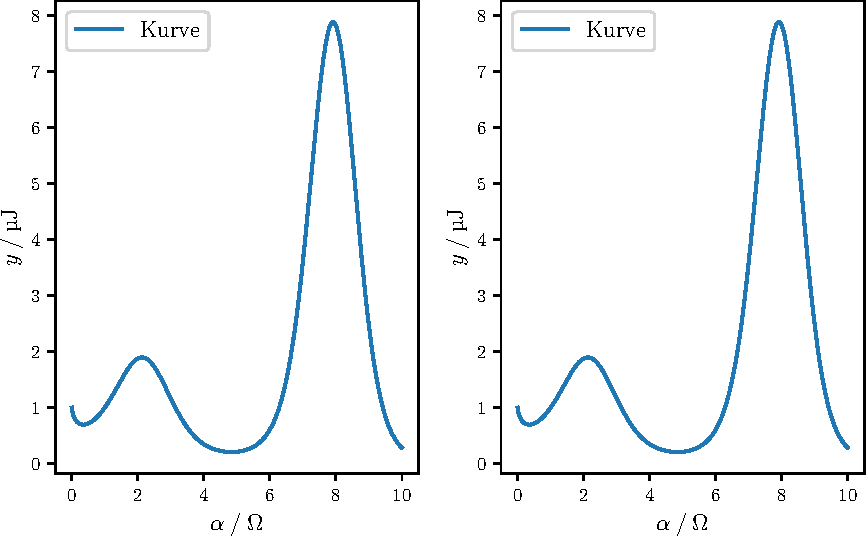
\includegraphics{build/plot.pdf}
  \caption{Laufzeiten in Abhängigkeit der Höhe des Acrylblocks abzüglich der Abstände zu den Störstellen und
  lineare Regression.}
  \label{fig:plot}
\end{figure}

Gleichung \eqref{eqn:lageFehler} lässt sich zu einer linearen Regressionsformel der Form
\begin{equation*}
  2h = c\cdot t + b
\end{equation*}
umformen. Mit der gegebenen linearen Regression aus \autoref{fig:plot} ergeben sich die Werte
\begin{align*}
  c &= (2756,01 \pm 9,33)\,\unit{\meter\per\second} \\
  b &= (-4,06 \pm 0,29)\cdot 10^{-3}\,\unit{\meter}\,. \\
\end{align*}


\subsection{Größe der der Störstellen}

Zusätzlich zu \autoref{tab:Laufzeiten1} werden die Laufzeiten zur Bestimmung der Tiefe und Dicke der Störstellen erneut von der anderen Seite des Acrylblocks
aufgenommen. Dies ist in \autoref{tab:Laufzeiten2} dargestellt.

\begin{table}[H]
  \centering
  \begin{tabular}{c c}
    \toprule
    Störstelle & $\symup{d}/\unit{\milli\meter}$ \\
    \midrule
     2 & 46,9 \\
     3 & 41,2 \\
     4 & 35,4 \\
     5 & 29,6 \\
     6 & 23,3 \\
     7 & 17,1 \\
     8 & 10,9 \\
    \bottomrule
  \end{tabular}
  \caption{Laufzeiten der Störstellen.}
  \label{tab:Laufzeiten2}
\end{table}
Aus Gleichung \eqref{eqn:lageFehler} kann die Strecke bis zur Störstelle berechnet werden. Aus den bestimmten Werte lassen sich
die Dicken der Störstellen bestimmen. Die Dicken der Störstellen sind in \autoref{tab:Abstand} zu finden.
\begin{table}
  \centering
  \begin{tabular}{c c}
    \toprule
    Störstellen & $\symup{d}/\unit{\milli\meter}$ \\
    \midrule
     2 & 2,65 \\
     3 & 1,97 \\
     4 & 4,86 \\
     5 & 4,73 \\
     6 & 5,18 \\
     7 & 5,83 \\
     8 & 6,37 \\
    \bottomrule
  \end{tabular}
  \caption{Dicke der Störstellen.}
  \label{tab:Abstand}
\end{table}







\subsection{B-Scan eines Acrylblocks}
Die Ergebnisse des B-Scans des Acrylblocks mit einer $2\,\unit{\mega\hertz}$-Sonde sind in \autoref{fig:Acryl1} und \autoref{fig:Acryl2} dargestellt.
\begin{figure}[H]
  \centering
  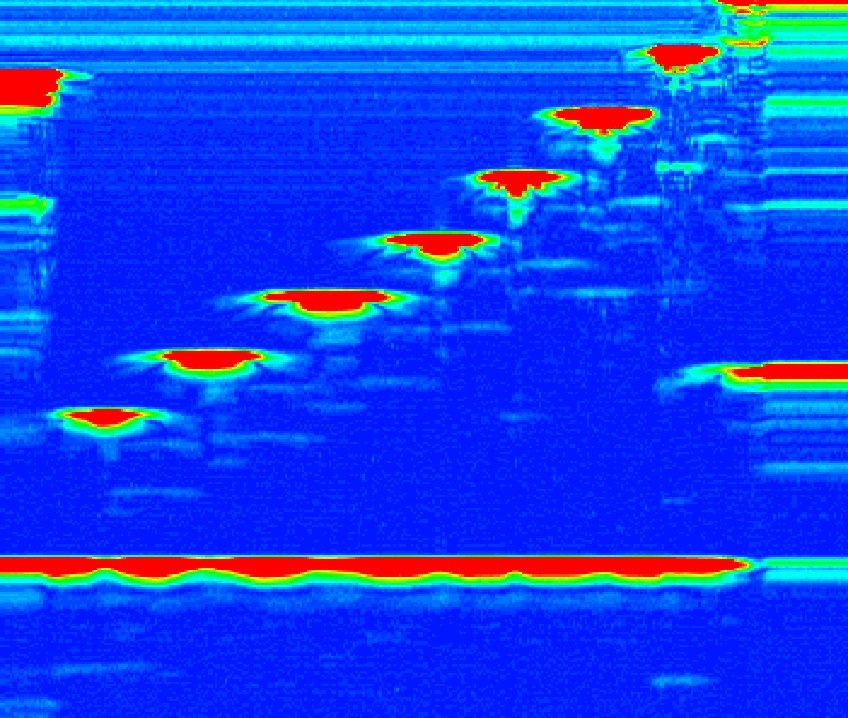
\includegraphics[width=0.7\textwidth]{data/oben.jpeg}
  \caption{B-Scan des Acrylblocks von oben.}
  \label{fig:Acryl1}
\end{figure}

\begin{figure}[H]
  \centering
  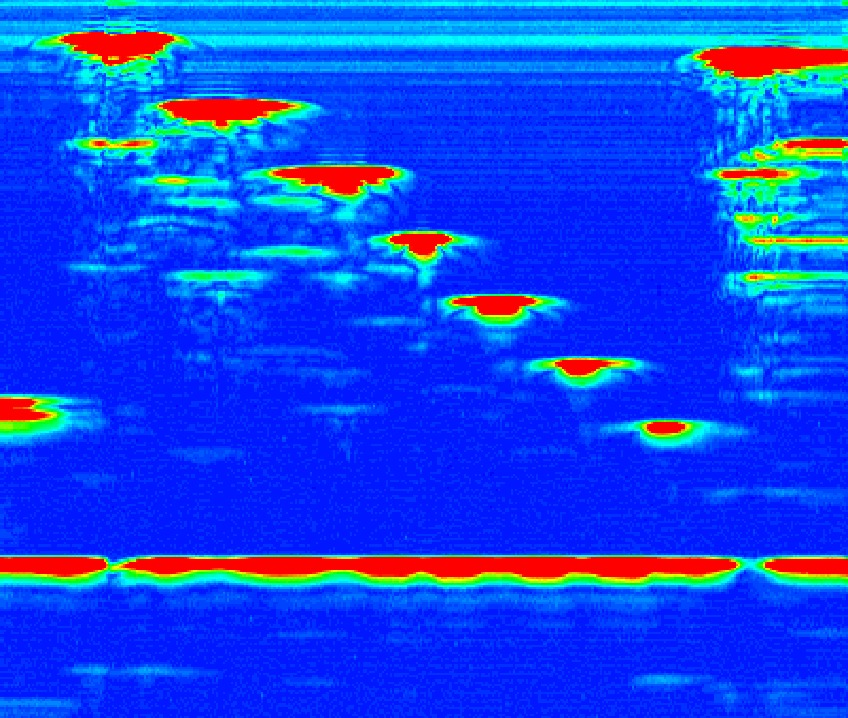
\includegraphics[width=0.7\textwidth]{data/unten.jpeg}
  \caption{B-Scan des Acrylblocks von unten.}
  \label{fig:Acryl2}
\end{figure}

Aus den Ergebnissen des B-Scans lassen sich nun die Lagen der Bohrungen bestimmen. Hierzu wird die Gleichung \eqref{eqn:lageFehler} verwendet.
Die ermittelten Werte sind in \autoref{tab:BScanDicke} dargestellt.

\begin{table}[H]
  \centering
  \begin{tabular}{c c c c c c}
    \toprule
    Störstellen & $t_{\symup{unten}}/\unit{\micro\second}$ & $t_{\symup{oben}}/\unit{\micro\second}$ & $s_{\symup{unten}}/\unit{\centi\meter}$ & $s_{\symup{oben}}/\unit{\centi\meter}$ & $d/\unit{\centi\meter}$ \\
    \midrule
     1 & 12 & 42 & 1,4 & 5,5 & 0,109 \\
     2 & 14 & 43 & 1,7 & 5,7 & 0,068 \\
     3 & 45 &  8 & 5,9 & 0,9 & 0,123 \\
     4 & 40 & 16 & 5,2 & 2,0 & 0,082 \\
     5 & 32 & 20 & 4,1 & 2,5 & 0,136 \\
     6 & 25 & 27 & 3,2 & 3,5 & 0,136 \\
     7 & 20 & 38 & 2,5 & 5,0 & 0,054 \\
     8 & 16 & 40 & 2,0 & 5,2 & 0,082 \\
     9 & 12 & 42 & 1,4 & 5,5 & 0,109 \\
    \bottomrule
  \end{tabular}
  \caption{Laufzeiten, Abstände und Dicken der Störstellen mit dem B-Scan ermittelt.}
  \label{tab:BScanDicke}
\end{table}


\subsection{B-Scan eines Brustmodels}

Beim Ertasten der Brust konnten zwei verschiedene Tumore erkannt werden. Diese konnten auch beide während des B-Scans gemessen werden. Eine der Messungen ist in
\autoref{fig:brust} dargestellt.
\begin{figure}[H]
  \centering
  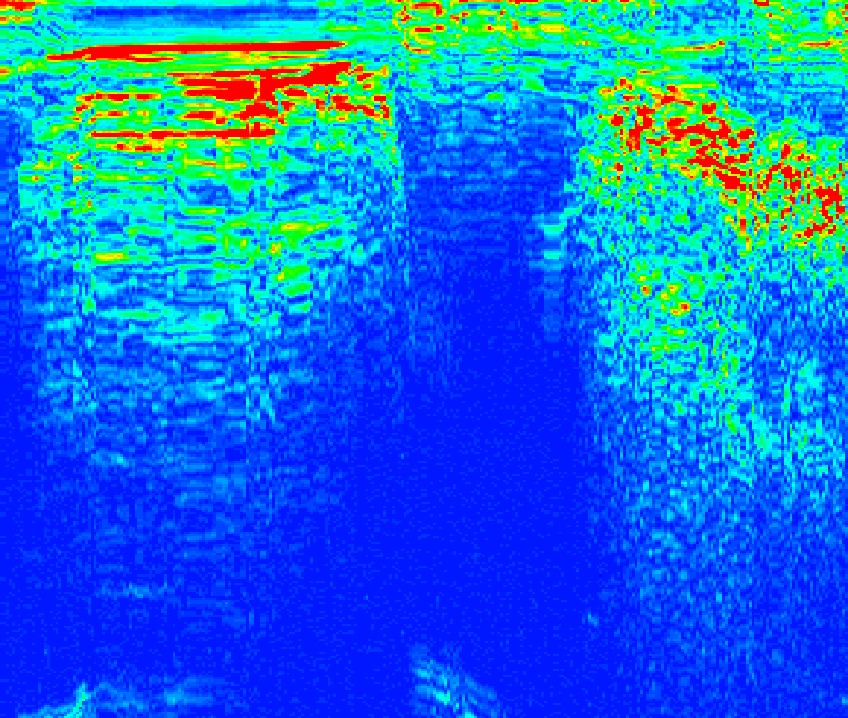
\includegraphics[width=\textwidth]{data/brust2.jpeg}
  \caption{B-Scan der Brust.}
  \label{fig:brust}
\end{figure}
Auf dem Scan ist deutlich zu erkennen, dass es sich um zwei seperate Tumore handelt. Es ist jedoch auch nach mehreren Versuchen nicht zu bestimmen, um welche Art des Tumors es
sich bei ihnen handelt. reli